\chapter{Análise e Projeto} \label{cap:espec}
% Introduzir capítulo, falar sobre análise e modelagem.
Este capítulo versa sobre a modelagem e planejamento do sistema. As próximas seções apresentarão a arquitetura do sistema, apresentando os componentes dele e suas relações; os requisitos, levantando as restrições técnicas e necessidades; a definição dos casos de uso, baseada nos objetivos do projeto e funcionalidades propostas; a prototipação das interfaces, a qual contemplará a comunicação entre usuário e sistema e por fim, a definição do modelo de entidade relacionamento, no qual o banco de dados será estruturado.  

\section{Arquitetura}
% explicar Cliente e Servidor, desenhar também.
Segundo Sommerville \citeyearpar{sommerville2003engenharia}, um modelo de arquitetura é uma representação visual da organização geral do sistema e ilustra as relações dos componentes que o compõe. Na Figura \ref{fig:arquitetura} está ilustrada a arquitetura deste projeto.

\begin{figure}[hb]
    \caption{Arquitetura do Pedal-to-Play.}
    \centerline{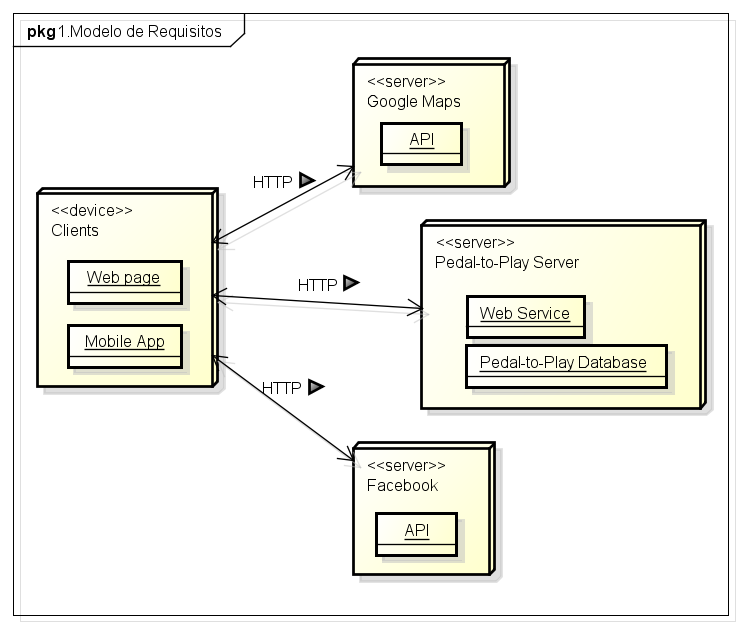
\includegraphics[width=30em]{figuras/arquitetura.png}}
    \label{fig:arquitetura}
\end{figure}

O modelo utilizado na organização dos componentes é o Cliente-Servidor,
no qual os processos de um cliente interagem com os processos de um servidor localizado em um domínio distinto. Os servidores gerenciam e compartilham recursos para seus clientes, podendo também ser clientes de outros servidores \cite{sommerville2003engenharia}.

\par Os clientes do Pedal-to-Play correspondem à aplicação \textit{mobile} e à \textit{web page}, esta última com acesso via navegador Web. Eles poderão requisitar serviços da API do Google Maps para visualização no mapa com as pedaladas monitoradas usando o aplicativo \textit{mobile}, assim como da API do Facebook para compartilhar ações realizadas no sistema. O \textit{web service} próprio do Pedal-to-Play será responsável pela autenticação do usuário e verificação da integridade dos dados enviados para serem salvos no banco de dados, este se localizará na mesma máquina do \textit{web service}.

\par A comunicação entre cliente e servidores utilizará o protocolo de mensagens HTTP e de comunicação TCP/IP. O \textit{web service} do Pedal-to-Play receberá requisições e enviará respostas no formato de arquivo JSON e seguirá a arquitetura REST. Ele não será responsável pelo envio de páginas Web (documentos HTML) ao cliente, as páginas serão dinâmicas e utilizarão requisições AJAX\footnote{Asynchronous Javascript and XML é uma termologia usada para simbolizar o emprego de diferentes tecnologias Web para uma aplicação rapidamente realizar atualizações sem necessidade que baixar a \textit{web page} inteira do servidor, somente requisitando as informações que são variáveis \cite{mdn2015ajax}.} para obtenção dos dados necessários para exibição correta ao usuário. 

\section{Requisitos}
Requisitos podem ser classificados como requisitos funcionais, os quais especificam o que o sistema deve ou não fazer e requisitos não funcionais, que compreendem restrições sobre as funcionalidades do sistema, tais como tempo, processos e padrões\cite{sommerville2003engenharia}. Os requisitos funcionais e não funcionais do Pedal-to-Play serão apresentados a seguir.

\subsection{Requisitos funcionais}
A primeira necessidade é possibilitar o \textbf{Monitoramento da atividade de ciclismo}, o qual deve ser feito através do rastreamento via geolocalização do \textit{smartphone} ou \textit{tablet} do usuário. Após a coleta dos dados da pedalada, o sistema deve calcular a distância do trajeto percorrido, velocidade média e tempo de duração.
\par
A segunda necessidade é o \textbf{Avatar virtual}. O avatar poderá ser customizado de acordo com os desejos do usuário e as peças disponíveis em relação ao nível do mesmo. A visualização do avatar deve estar presente na tela inicial da aplicação.
Ele é composto por dois elementos: o ciclista e a bicicleta. O ciclista é dividido em 3 partes interligadas: cabelo, rosto (olhos, boca e nariz) e equipamentos. Os equipamentos incluem: capacete, \textit{jersey}(malha) e \textit{shorts}, calçados, luva e óculos. Cada nível cumprido torna disponível ao usuário um novo modelo de bicicleta e um novo equipamento. 
\par
A terceira necessidade é a \textbf{Motivação para prática da atividade física}. O Pedal-to-Play deve propor desafios ao usuário, através destes possibilitar a obtenção de recompensas de acordo com os resultados obtidos. As recompensas envolvem novos itens para customizar o avatar. 
\par 
Também para promover motivação, o sistema deve possibilitar o compartilhamento em redes sociais dos feitos dentro da aplicação, tais como o cumprimento de desafios, a inclusão de pedaladas e a customização do avatar. 
\par 
A quarta necessidade é o \textbf{Gerenciamento de usuários}. Esta necessidade envolve a manutenção do cadastro dos usuários; a autenticação deles no sistema e a visualização de informações de desempenho, tais como: nível, distâncias percorridas, velocidade, tempos de atividade e total de distância já percorrida.
\par
A manutenção do cadastro de usuário envolve algumas regras de negócio, tais como:
o email dever ser usado como nome de usuário para autenticação e deverá estar no formato válido de email (\textit{usuario@subdomínio.domínio}); a senha do usuário deve conter de 6 a 30 caracteres e deve ser criptografada logo após a entrada dela no sistema; para o formulário de cadastro ser válido e concluído é necessário que a senha e a senha de confirmação sejam idênticas; os campos de email, senha e confirmação de senha são obrigatórios para cadastro de um novo usuário e não se deve habilitar o registro de um email já cadastrado. 
    
\subsection{Requisitos não funcionais}
O \textit{software} deve utilizar tecnologias do desenvolvimento Web, pois um dos objetivos dele é ser multiplataforma.
\par
O sistema operacional \textit{mobile} suportado deverá ser o Android (a partir da versão 4.1, pois esta é a menor versão disponível para teste nos dispositivos disponíveis e também a que apresenta os requisitos mínimos de todas as tecnologias a serem implementadas). O sistema não terá versão para iOS nativo devido à necessidade de um Apple ID e uma conta de desenvolvedor, a qual para ser mantida ativa é necessário pagar uma anuidade.
\par
Para customização do avatar também é necessário que o dispositivo suporte SVG \textit{inline}\footnote{SVG é um formato de imagens vetoriais baseado em XML\cite{w3c2011svg}}.
\par
Os navegadores suportados para acesso à \textit{web page} deverão ser o Chrome, Firefox e Internet Explorer (a partir da versão 10), pois estes suportam as tecnologias que precisarão ser implementadas no \textit{software}.
\par
A manutenibilidade e portabilidade proporcionada pela implementação de \textit{frameworks}. Tais como, o Bootstrap (versão 3.3.5), para desenvolvimento de \textit{web pages} responsivas e adaptáveis a múltiplos tamanhos de tela; o AngularJS (versão 1.4.6) para o desenvolvimento da parte lógica no cliente usando JS; o Phonegap/Cordova (versão 5.2.0) para compilação do \textit{software} para a plataforma Android e acesso aos recursos de \textit{hardware} dos dispositivos
e o micro \textit{framework} Slim\footnote{\url{http://www.slimframework.com/}} de PHP, o qual é especializado no desenvolvimento de Web APIs e propõe-se a facilitar a implementação das rotas do \textit{web service} (URLs para requisição de recursos do servidor) e gerenciamento de autenticação.
\par
O banco de dados deve ser MySQL e hospedado junto ao servidor, qual deve usar o serviço de hospedagem em nuvem do Red Hat OpenShift. Este serviço possui um plano de uso básico gratuito com uma máquina virtual Linux; suporte a várias linguagens de programação, \textit{frameworks}, banco de dados e servidores Web; integração com Git\footnote{\url{https://git-scm.com/}}; servidores fisicamente localizados na América escalonamento automático da aplicação e acesso SSH.

\pagebreak

\section{Diagrama de Caso de Uso}
Os casos de uso são técnicas de obtenção de requisitos baseadas na representação visual de interações entre componentes de um cenários \cite{sommerville2003engenharia}. O diagrama de Casos de Uso do Pedal-to-Play se encontra na Figura \ref{fig:usecase}.

\begin{figure}[h]
\begin{minipage}{1.0\textwidth}
    \captionof{figure}{Diagrama de Caso de Uso.}
    \centerline{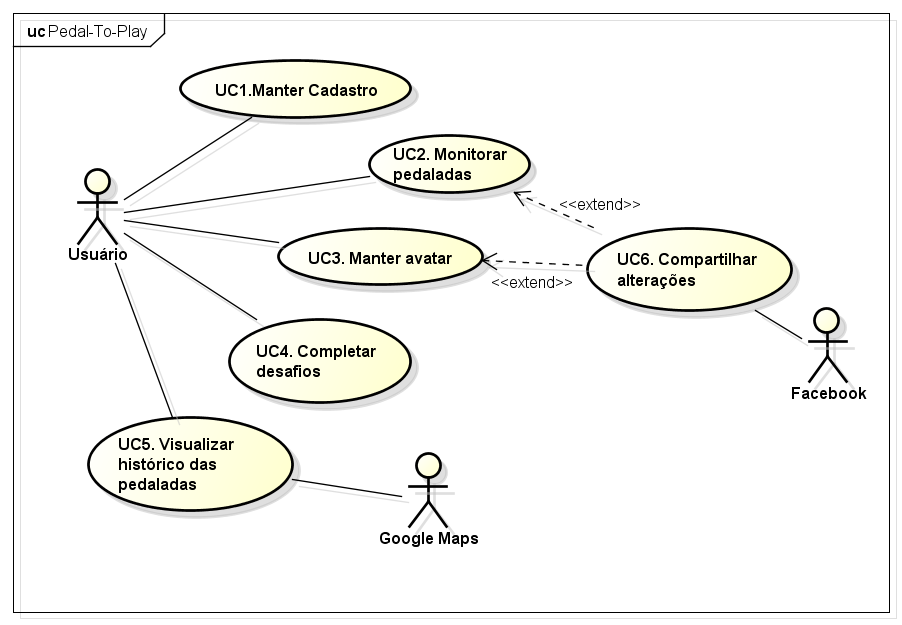
\includegraphics[width=28em]{figuras/useCaseDiagram.png}}
    \label{fig:usecase}
\end{minipage}
\end{figure}

Neste diagrama se encontram seis casos de uso extraídos a partir das necessidades apresentadas nos requisitos funcionais e suas funcionalidades. O caso de uso UC1 está vinculado à necessidade de gerenciamento de usuários; o UC2 à necessidade de monitoramento de atividades; o UC3 à necessidade do avatar e o UC4 e o UC6, à necessidade de motivação. O caso de uso UC5 representa a funcionalidade para visualização das pedaladas monitoradas no Pedal-to-Play e a conexão com a API do Google Maps, o qual é um ator secundário que tem seus serviços requisitados para visualização gráfica dos caminhos das pedaladas. O Facebook também é um ator secundário, o qual pode fornecer seus serviços de compartilhamento de informação. As relações entre o UC6 e os outros casos de uso se classificam como de extensão, pois é uma funcionalidade opcional proposta dentro das funcionalidades de customização do avatar e monitoramento de pedaladas.

\section{Protótipos de telas}
A prototipação de interface gráficas é uma peça fundamental no processo de desenvolvimento de interfaces \cite{sommerville2003engenharia}. Os protótipos de telas do Pedal-to-Play tem o objeto de orientar o desenvolvimento das interfaces gráficas com o usuário (GUI), de modo a detalhar quais elementos devem compô-la, a função de cada um e o posicionamento deles, assim como cores e ícones.  

\subsection{Autenticação de usuário}
Os protótipos da GUI de autenticação compreendem as telas de \textit{login} e cadastro no sistema, as quais podem ser vistas nas Figuras \ref{fig:loginProto} e \ref{fig:signupProto}, respectivamente. Essas GUI tiveram como inspiração as interfaces de autenticação dos aplicativos Strava e Runtastic. 
\par
O botão superior direito em ambas as telas deve permitir a navegação de uma para a outra. O botão inferior deve confirmar os dados preenchidos no formulário e concluir as operações, redirecionando para a tela inicial do sistema em caso dos dados serem aprovados.

\begin{figure}
\centering
\begin{minipage}{.5\textwidth}
  \captionof{figure}{Protótipo da tela\\de login.}
  \centerline{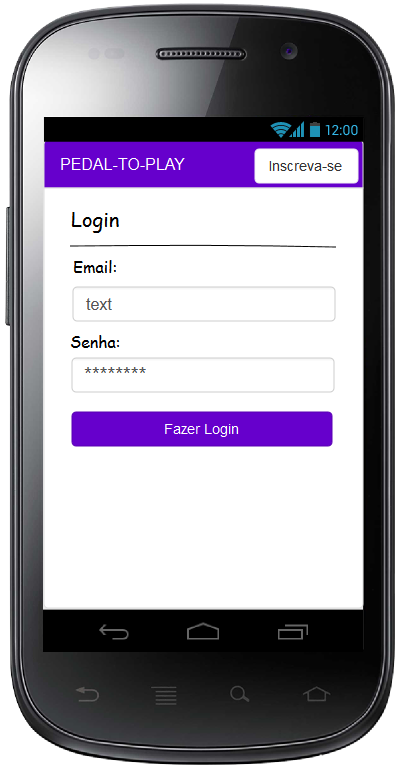
\includegraphics[width=0.7\linewidth]{figuras/Login.png}}
  \label{fig:loginProto}
\end{minipage}%
\begin{minipage}{.5\textwidth}
  \captionof{figure}{Protótipo da tela\\de cadastro.}
  \centerline{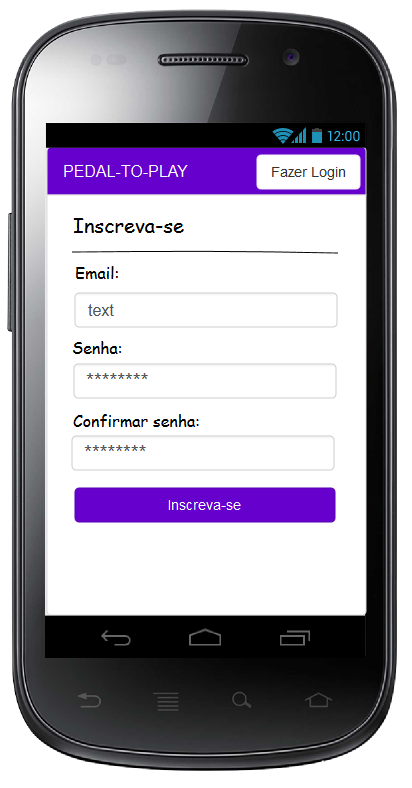
\includegraphics[width=0.7\linewidth]{figuras/Inscreva-se.png}}
  \label{fig:signupProto}
\end{minipage}
\end{figure}

\subsection{Monitoramento de atividade de ciclismo}
Os protótipos do monitoramento de pedalada envolvem as GUI de monitoramento em si (Figura \ref{fig:trackProto}) e a de visualização de pedaladas já monitoradas e registradas no sistema (Figura \ref{fig:recordsProto}). As inspirações para a prototipação dessas interfaces foram, novamente, os aplicativos Strava e Runtastic. 
\par
No protótipo da interface de monitoramento deve haver a opção de gravar a pedalada, a qual deve iniciar o processo de monitoramento via geolocalização do dispositivo \textit{mobile} do usuário. Durante a gravação, as medidas de distância, velocidade e duração devem atualizar-se em tempo real e devem ser exibidas as opções ilustradas na parte direita da Figura \ref{fig:trackProto}. O botão com o ícone de cadeado (botão central dos três inferiores) deve bloquear os outros botões (com o objetivo de evitar toques acidentais), assim desbloqueá-los, permitindo que o usuário possa pausar a gravação ou pará-la. Ao pará-la, o \textit{dialog} para salvar atividade deve ser exibido, nele o usuário pode optar por descartar a gravação ou salvá-la.
\par
O protótipo da interface de visualização do histórico de pedaladas ilustra a visualização dos trajetos de uma pedalada através de um mapa. O histórico de pedaladas remete a lista localizada à direita do mapa. A cima do mapa deve encontrar-se as medidas totais extraídas da pedalada em questão. 

\begin{figure}
\begin{minipage}{1.0\textwidth}
    \captionof{figure}{Protótipo da tela de monitoramento de pedalada.}
    \centerline{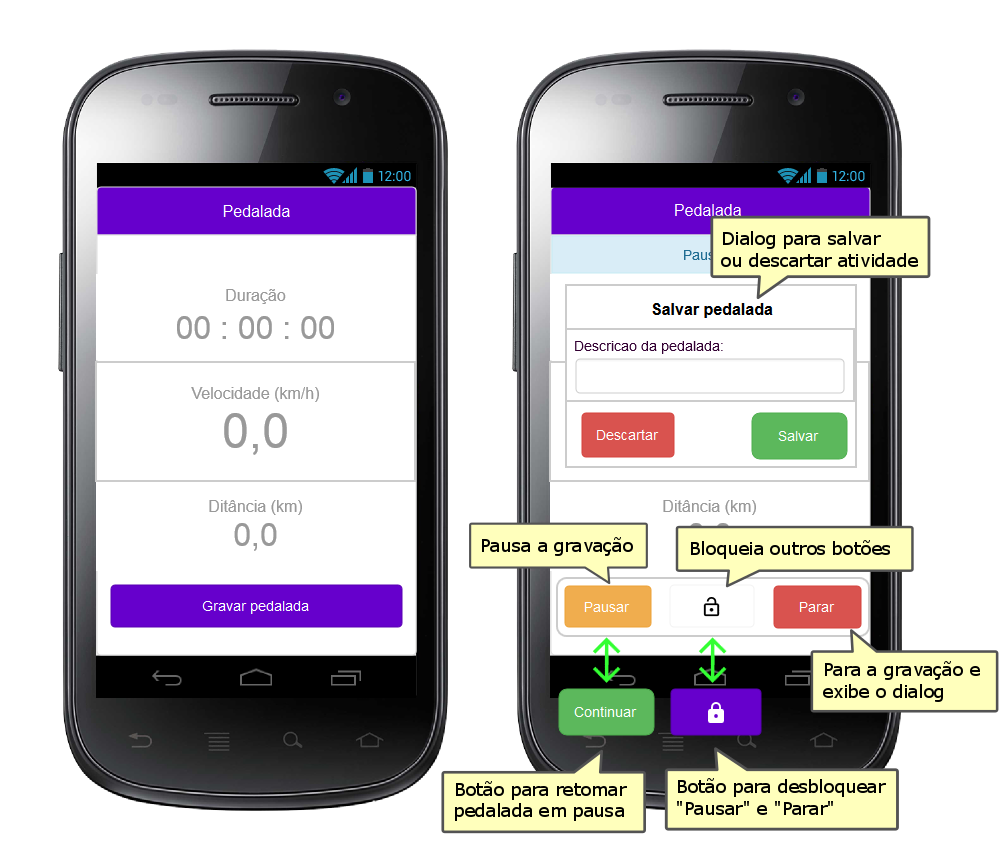
\includegraphics[width=30em]{figuras/Monitoramento.png}}
    \label{fig:trackProto}
\end{minipage}
\end{figure}

\begin{figure}
\begin{minipage}{1.0\textwidth}
    \captionof{figure}{Protótipo da tela de histórico de pedaladas.}
    \centerline{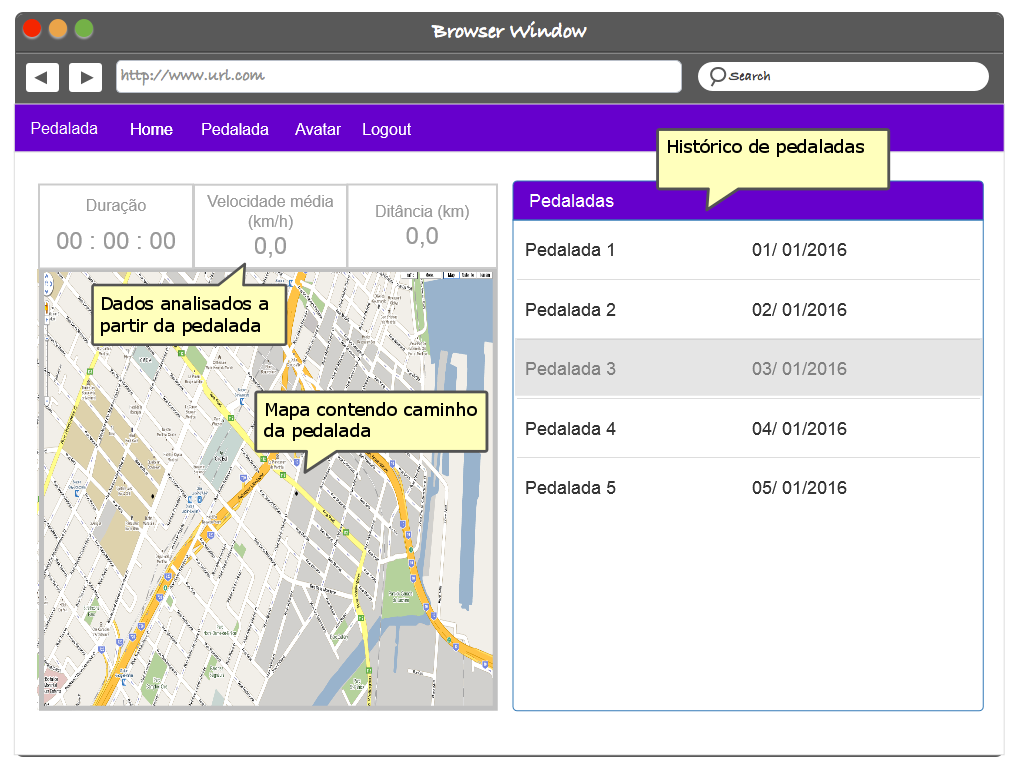
\includegraphics[width=30em]{figuras/Historico.png}}
    \label{fig:recordsProto}
\end{minipage}
\end{figure}

\pagebreak

\subsection{Avatar virtual}
Os protótipos das GUI do sistema do avatar foram inspirados nas interfaces de aplicativos \textit{mobile} existentes no mercado específicos desta temática. Os aplicativos foram escolhidos com base na popularidade deles na Google Play (loja virtual do Google com aplicativos para Android e mídias diversas). Eles são os seguintes: o BuddyPoke\footnote{https://play.google.com/store/apps/details?id=com.buddypoke.buddypoke}; o WeeMee\footnote{https://play.google.com/store/apps/details?id=novoda.weeworld} e o FaceQ\footnote{https://play.google.com/store/apps/details?id=com.miantan.myoface}.
\par
As Figuras \ref{fig:homeProto} e \ref{fig:avatarProto} são os protótipos das interfaces do sistema do avatar virtual, sendo a da esquerda também a tela inicial da aplicação (\textit{Home}).

\begin{figure}[h]
\centering
\begin{minipage}{.5\textwidth}
  \captionof{figure}{Protótipo da tela\\inicial da aplicação.}
  \centerline{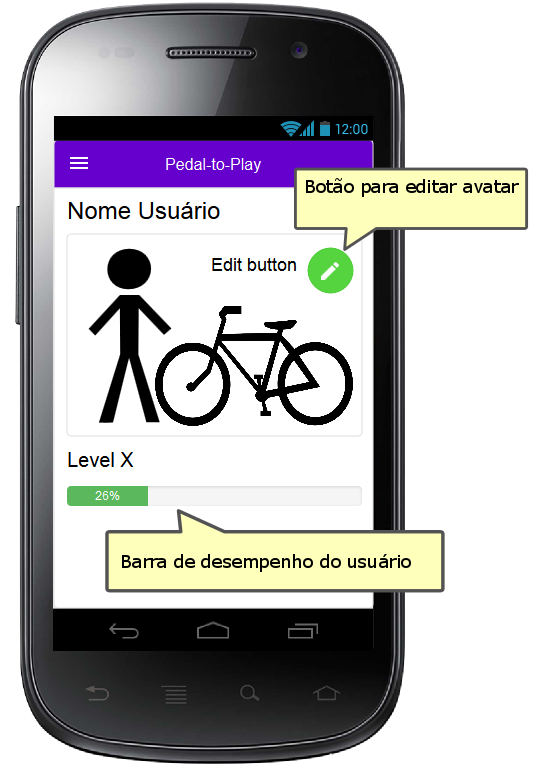
\includegraphics[width=.8\linewidth]{figuras/Visualizacao.png}}
  \label{fig:homeProto}
\end{minipage}%
\begin{minipage}{.5\textwidth}
  \captionof{figure}{Protótipo da tela de\\customização de avatar.}
  \centerline{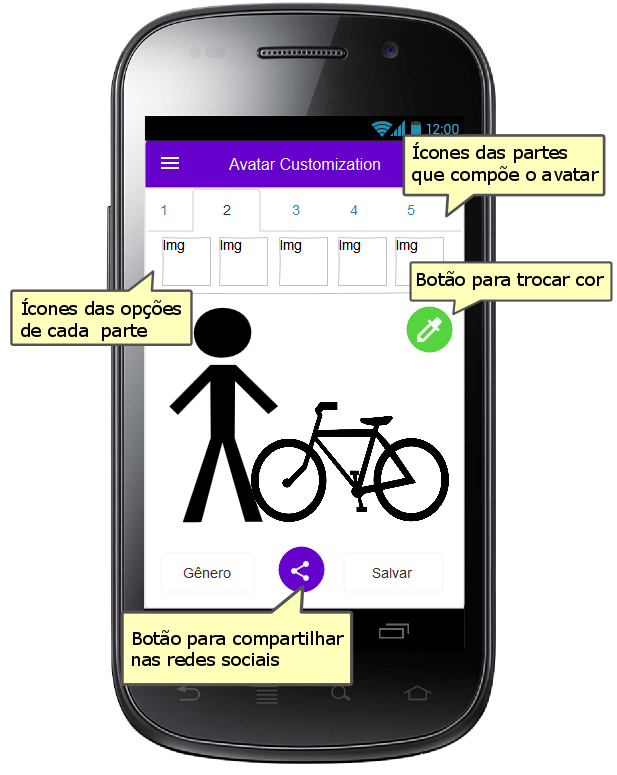
\includegraphics[width=.9\linewidth]{figuras/Customizacao.png}}
  \label{fig:avatarProto}
\end{minipage}
\end{figure}

A tela de \textit{Home} deve possuir, além do avatar, uma barra de progresso que ilustra o desenvolvimento do usuário na atividade de ciclismo, baseado no medida de distância total acumulada. O botão para editar o avatar deve redirecionar para a tela de customização (à direita). A tela de customização do avatar deve ser composta pelos elementos necessários para realizar alterações no avatar, assim como o botão de compartilhamento em redes sociais.

\section{Diagrama de Entidade Relacionamento}
Diagramas de Entidade Relacionamento são utilizados para definir o modo lógico dos dados que serão processados e armazenados pelo sistema. Eles apresentam as entidades que compõe o \textit{software}, seus atributos e o relacionamento entre elas. Esses diagramas servem como base para estruturação e especificação do banco de dados do sistema \cite{sommerville2003engenharia}. A Figura \ref{fig:ermodel} corresponde ao Diagrama de Entidade Relacionamento do Pedal-to-Play.

\begin{figure}
\begin{minipage}{1.0\textwidth}
    \captionof{figure}{Diagrama Entidade Relacionamento.}
    \centerline{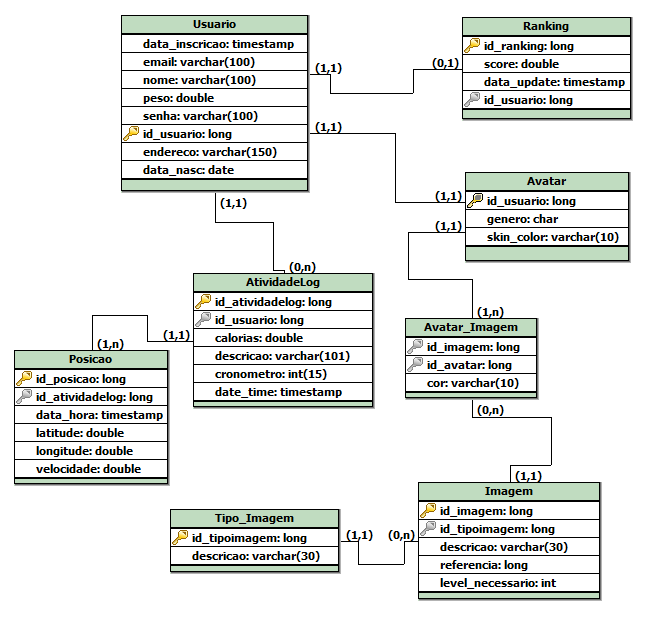
\includegraphics[width=26em]{figuras/er.png}}
    \label{fig:ermodel}
\end{minipage}
\end{figure}

A entidade \textit{User} corresponde ao cadastro de usuário no sistema, ela é o centro do sistema e se relaciona diretamente com as entidades \textit{Ranking}, \textit{Avatar} e \textit{AtividadeLog}. A entidade \textit{Ranking} possui os atributos relacionados à quantificação dos pontos (\textit{score}) de cada usuário, esses pontos determinam o nível em que ele está e são baseados na distância acumulada por todas as pedaladas registradas por ele. O registro de pedaladas e seus dados remetem à entidade \textit{AtividadeLog}, cada registro desta entidade representa uma pedalada e possui relação com vários itens da entidades \textit{Posição}. Cada item da entidade \textit{Posição} refere-se a um elemento retornado pela tecnologia de geolocalização.
\par
A entidade \textit{Avatar} remete aos dados dos avatares virtuais dos usuários. Ela é normalizada nas entidades \textit{Imagem}, a qual se relaciona com a entidade \textit{Tipo\_Imagem} (esta refere-se à categoria do objeto ilustrado na imagem, exemplo: bicicleta, vestimenta ou rosto.) e \textit{Avatar\_Imagem}, sendo esta uma entidade de relacionamento para vincular um avatar e suas várias imagens, assim como uma imagem e os diversos avatares que possam vir a fazer uso dela (tipo de relacionamento \textit{Many-to-Many}).  

\section{Conclusões}
Neste capítulo foram apresentadas as técnicas de análise e projeto do Pedal-to-Play. Incluiu a descrição da arquitetura do sistema, o levantamento de requisitos, a diagramação de casos de uso e de entidade relacionamento, assim como a prototipação de interfaces com o usuário.
\par
No capítulo seguinte será dissertada a implementação dos itens analisados e projetados nas sessões anteriores. O que incluí o Módulo de Autenticação, do Avatar Virtual, de Monitoramento e Registro de Pedaladas e de Desafios.

% ~~~~~~~~~~~~~~~~~~~~~~~~~~~~~~~~~~~~~~~~~~~~~~~~~~~~~~~~~~~~~~~~~~~~~~~~ %

\chapter{Implementação} \label{cap:desenv}
% Introduzir capítulo, falar sobre Implementação.
A etapa de implementação caracteriza-se no processo de projetar os módulos do sistema a partir dos requisitos e arquitetura, adequando estes projetos ao ambiente de desenvolvimento e então, desenvolvendo a solução técnica \cite{openupDevelopment}. 
\par
O processo adotado para desenvolvimento do Pedal-to-Play foi o de Desenvolvimento Incremental, no qual o desenvolvimento do \textit{software} é divido em entregas com prazos curtos, chamadas incrementos, os quais reúnem um conjunto de funcionalidades \cite{sommerville2003engenharia}. Os incrementos do Pedal-to-Play sãos os casos de uso definidos no levantamento de requisitos e cada um deles foi convertido em um módulo do sistema.
\par
Os módulos do Pedal-to-Play estruturam-se no padrão de projeto MVC (Model-View-Controller). Este padrão teve suas origens no Smalltalk e tem como objetivo a separação da apresentação e da lógica do \textit{software} em si. O modelo (Model) corresponde às entidades que compõe o sistema e ao gerenciamento de dados; as visões (Views) referem-se às interfaces do sistema, sejam elas gráficas, linhas de comando ou APIs e os controladores (Controller) são objetos manipuladores das visões e gerenciadores de eventos, os quais atuam como pontes entre o modelo e as visões \cite{burbeck1992applications}. 

\section{Módulo de Autenticação de Usuário}
O módulo de autenticação remete à necessidade de manter um cadastro de usuário e identificá-lo no sistema. Os dados necessários para identificar o usuário são seu email, senha, identificador numérico único (ID) e \textit{token} (sequência de caracteres gerada automaticamente pelo servidor).
\par
A senha do usuário é capturada na GUI de cadastro ou \textit{login} e, ainda no lado do cliente, é criptografada em MD5\footnote{MD5 é um algoritmo de \textit{hashing} que a partir de uma entrada de texto gera uma saída de 128 bits. Presume-se que é computacionalmente inviável produzir uma saída igual para duas mensagens diferentes e descobrir o texto original, tendo somente a saída gerada \cite{rfc1321MD5}} utilizando o módulo de AngularJS, Angular-MD5\footnote{\url{https://github.com/gdi2290/angular-md5}}.
\par
Quando um novo usuário é cadastrado e seus dados são verificados, um \textit{token} e ID são gerados pelo servidor e enviados para o cliente. O \textit{token} e ID são agregados aos cabeçalhos HTTP de todas as requisições feitas pelo cliente para com o servidor, a fim de identificar o usuário que deseja executar alterações em seus dados. Optou-se por usar esta forma de autenticação no lugar da senha e email do usuário para evitar o tráfego excessivo destas informações pela Internet. 
\par
A Figura \ref{fig:authSequence} ilustra como o usuário é autenticado no sistema e identificado em suas requisições ao servidor. E a Figura \ref{fig:authclasses} apresenta o \textit{design} do módulo de autenticação baseado no padrão MVC.

\begin{figure}
\begin{minipage}{1.0\textwidth}
    \captionof{figure}{Processo de autenticação de usuário.}
    \centerline{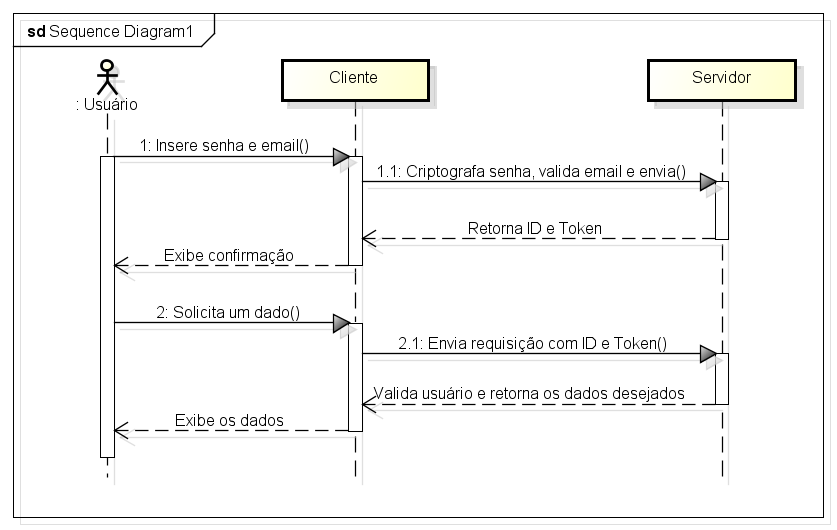
\includegraphics[width=30em]{figuras/authSequence.png}}
    \label{fig:authSequence}
\end{minipage}
\end{figure}

\begin{figure}
\begin{minipage}{1.0\textwidth}
    \captionof{figure}{Diagrama de classes simplificado do Módulo de Autenticação.}
    \centerline{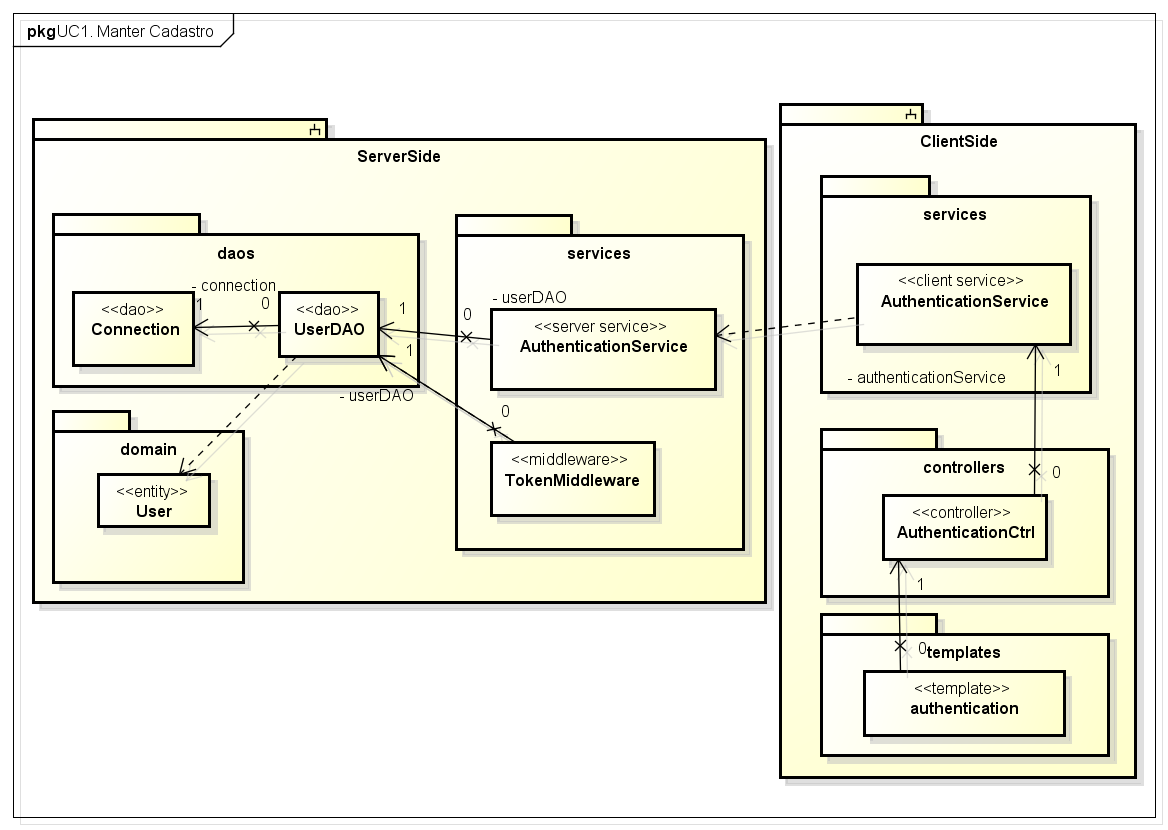
\includegraphics[width=35em]{figuras/authClasses.png}}
    \label{fig:authclasses}
\end{minipage}
\end{figure}

No lado do cliente, os objetos de estereótipo  \textit{template} representam as GUI do sistema e são gerenciados pelos objetos de estereótipo  \textit{controller}. Os \textit{controllers} são responsáveis pelo dinamismo das GUI e, especialmente no módulo de autenticação, a criptografia da senha do usuário. Eles também se comunicam com os objetos de estereótipo  \textit{client service}, cuja responsabilidade é verificar a integridade dos dados de entrada e providenciar o armazenamento ou resgate deles. Os \textit{client service} são a ponte de tráfego de dados entre cliente e servidor. 
\par
O armazenamento de dados no lado do cliente é feito usando o armazenamento local da Web \footnote{\url{http://www.w3.org/TR/webstorage/\#the-localstorage-attribute}}, o acesso a este recurso no Pedal-to-Play é feito pelo módulo de AngularJS, Angular-local-storage\footnote{\url{https://github.com/grevory/angular-local-storage}}.
\par
No lado do servidor, os objetos de estereótipo  \textit{server service} se comportam do mesmo modo dos \textit{client services}, mas além da verificação e tráfego dos dados, os \textit{server services} relacionam-se com os \textit{data access objects} (DAOs). Os DAOs têm a responsabilidade de gerenciar o banco de dados do sistema. Eles se relacionam com os objetos de estereótipo  \textit{domain}, os quais são referências às tabelas do banco de dados.
\par
O objeto \textit{middleware} é um caso especial, sua responsabilidade é validar o cliente que requisitou um serviço do servidor, através do ID e \textit{token} do usuário. \textit{Middleware} é um recurso do \textit{framework} Slim que permite a interceptação de toda requisição ao servidor com o objetivo de fazer uma pré verificação dos dados. No caso do TokenMiddleware, se os dados do usuário forem válidos, a requisição segue seu fluxo normalmente. Do contrário, é disparado um erro para o cliente, com \textit{status} 401 (\textit{Unauthorized})\footnote{\url{http://www.w3.org/Protocols/rfc2616/rfc2616-sec10.html}}.

\section{Módulo de Monitoramento e Registro de Pedaladas}
O módulo de monitoramento compreende dois casos de uso, o monitoramento de uma atividade de ciclismo (usando geolocalização) e a visualização do histórico de atividades passadas. A visualização do histórico pode ser acessada em qualquer dispositivo com a cesso a Internet e um navegador Web (levando em consideração os navegadores suportados pelo sistema), no entanto, o monitoramento é uma função exclusiva dos dispositivos \textit{mobile}, pois utiliza a API do Cordova e seu \textit{plugin} de geolocalização\footnote{\url{https://github.com/apache/cordova-plugin-geolocation}} para acesso ao GPS do dispositivo.
\par
Além do \textit{plugin} de geolocalização, este módulo utiliza os \textit{plugins} do Cordova, Cordova-plugin-network-information\footnote{\url{https://github.com/apache/cordova-plugin-network-information}} e Cordova-diagnostic-plugin\footnote{\url{https://github.com/dpa99c/cordova-diagnostic-plugin}}. Os \textit{plugins}, respectivamente, permitem a verificação do \textit{status} da rede do dispositivo (se este está conectado à Internet e qual o tipo da rede) e permitem verificar se os recursos do dispositivo estão, ou não, ativos (para o monitoramento é importante sabe se o GPS está ativo).
\par
Para desenvolvimento da solução técnica do monitoramento por geolocalização, tomou-se como referência os tutoriais de Brian Ford (desenvolvedor filiado ao Google, envolvido diretamente no projeto do AngularJS)\citeyearpar{fordCordova} e de Mortimer\citeyearpar{mortimer2012}. Ford descreveu como utilizar a plataforma Cordova em conjunto com o \textit{framework} AngularJS e Mortimer descreveu como desenvolver uma aplicação básica para rastrear atividades do usuário usando os recursos de geolocalização do Cordova.
\par
Baseando-se em Ford e Mortimer, o monitoramento de atividades do Pedal-to-Play foi implementado da seguinte maneira: verifica-se a disponibilidade do Cordova, se disponível, verifica-se se o GPS está ativo, se sim, começa o monitoramento. Durante o monitoramento, a GUI se atualiza com os valores retornados da API de geolocalização e exibe para o usuário as opções de Parar e Pausar a atividade. Se o usuário solicitar pausar, pause-se o fluxo até segunda ordem. Se solicitar parar, termina o fluxo e pergunta-se ao usuário se deseja salvar ou descartar a atividade monitorada. Caso a escolha seja salvar, o lado cliente verifica os dados e os envia para o servidor e caso seja descartar, encerra-se o fluxo.
\par
Caso perca-se o sinal do GPS ou aconteçam erros consecutivos na API de geolocalização, pausa-se o monitoramento até que a situação normalize e caso o dispositivo esteja sem conexão com a Internet quando o usuário solicitar o salvamento de uma atividade, a aplicação cliente salva localmente em uma fila. Quando uma atividade é enviada com sucesso ao servidor, a aplicação envia o conteúdo da fila (se está não estiver vazia) em seguida.
\par
No lado do servidor, verificam-se os dados novamente e a autenticação do usuário antes de salvar a atividade. O salvamento se dá pela interpretação da mensagem vinda do cliente, a qual contém as características da atividade (descrição, duração e data) e o trajeto percorrido, composto por um conjunto de objetos \textit{Position}. O objeto \textit{Position} é o retorno da API de geolocalização do Cordova em cada iteração do ciclo de monitoramento. Ele é especificado segundo a W3C e possui os seguintes atributos:
\begin{itemize}
\item \textit{timestamp}: Data e hora do sistema.
\item \textit{coords}: arranjo de coordenadas.
    \begin{itemize}
        \item \textit{latitude}: Latitude em graus decimais.
        \item \textit{longitude}: Longitude em graus decimais.
        \item \textit{altitude}: Altura da posição em metros.
        \item \textit{accuracy}: Nível de precisão da latitude e longitude em metros.
        \item \textit{altitudeAccuracy}: Nível de precisão da altitude em metros. 
        \item \textit{heading}: Direção da viagem, especificado em graus contando no sentido horário em relação ao norte verdadeiro.
        \item \textit{speed}: A velocidade atual do aparelho em relação ao chão, especificado em metros por segundo.
    \end{itemize}
\end{itemize}

\par
A Figura \ref{fig:trackingActivity} ilustra o fluxo principal de monitoramento, desconsiderando possíveis falhas, e a Figura \ref{fig:trackingClasses} apresenta o \textit{design} do módulo de Monitoramento.

\begin{figure}
\begin{minipage}{1.0\textwidth}
    \captionof{figure}{Fluxo principal de Monitoramento de Pedalada.}
    \centerline{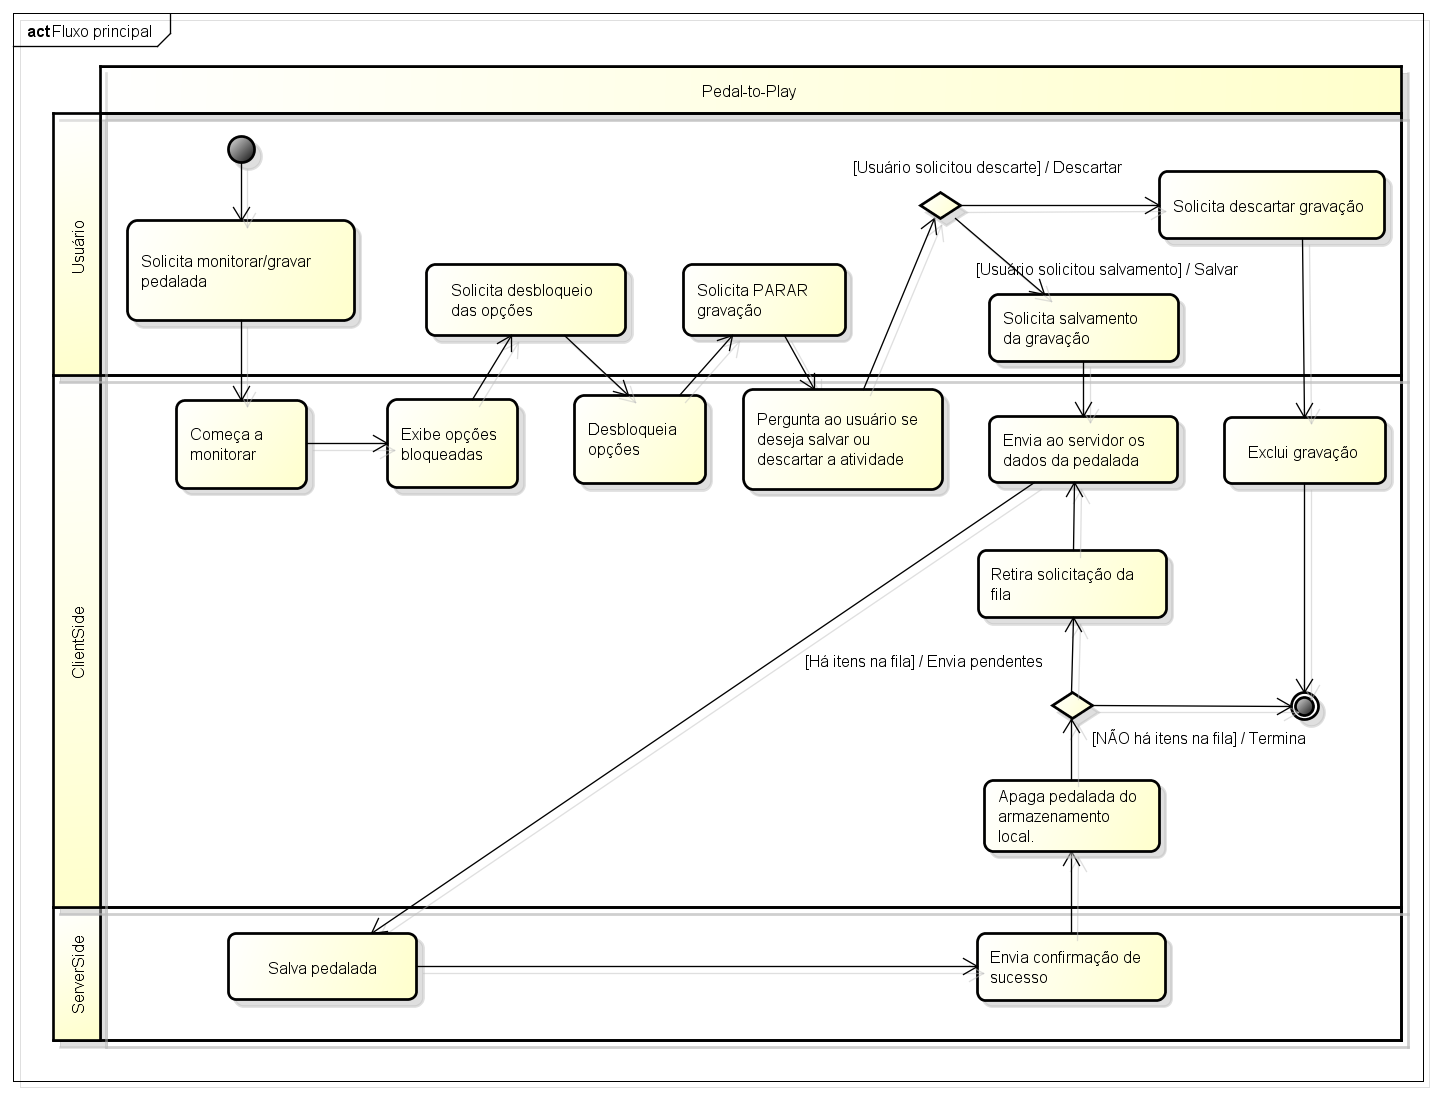
\includegraphics[width=35em]{figuras/trackingActivity.png}}
    \label{fig:trackingActivity}
\end{minipage}
\end{figure}

\begin{figure}
\begin{minipage}{1.0\textwidth}
    \captionof{figure}{Diagrama de classes simplificado do Módulo de Monitoramento de Pedalada.}
    \centerline{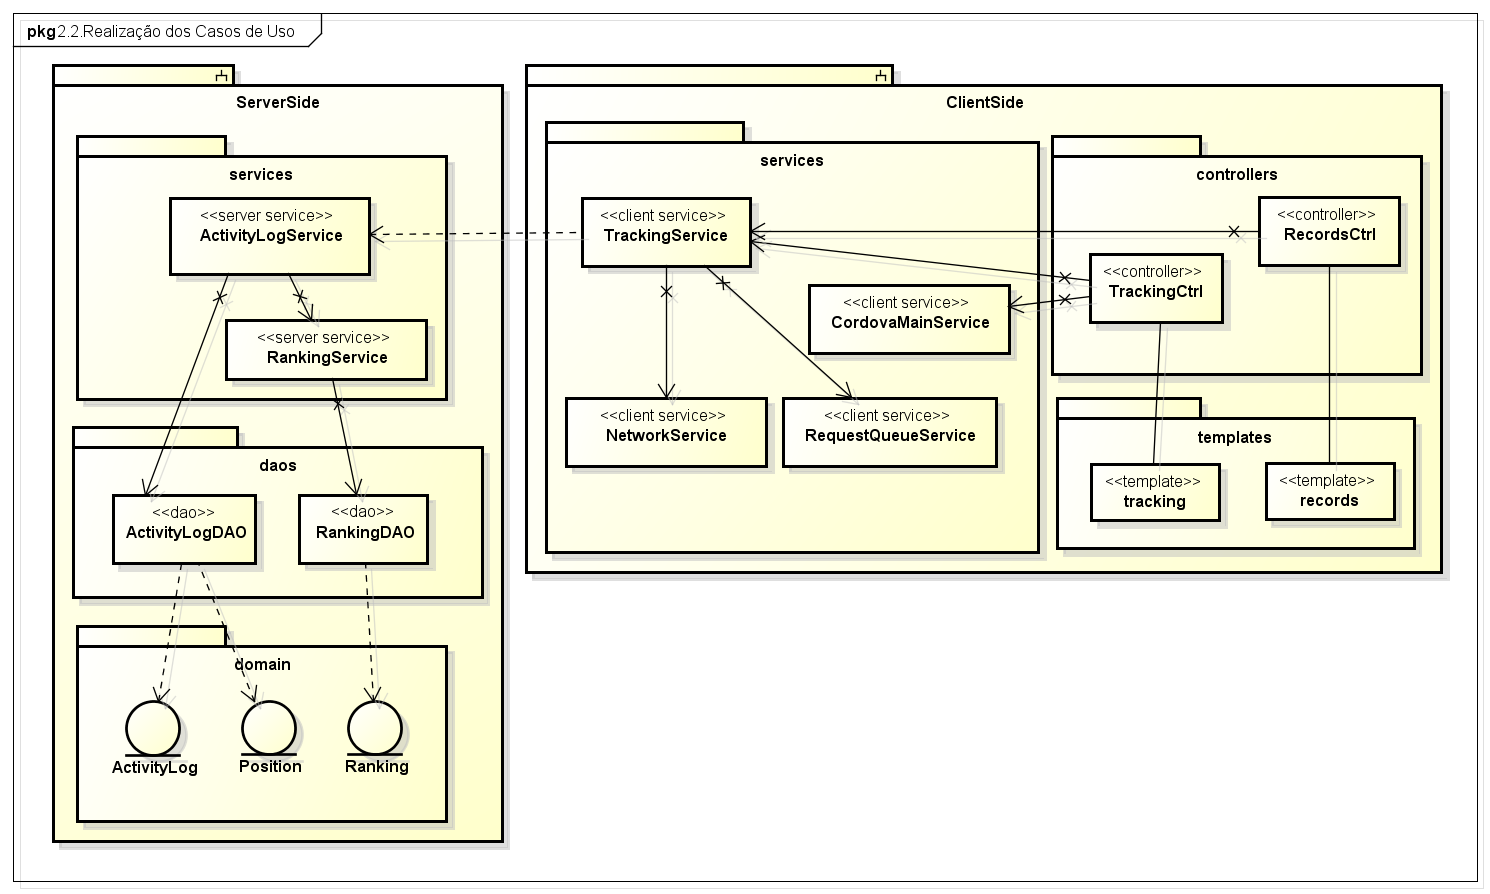
\includegraphics[width=35em]{figuras/trackingClasses.png}}
    \label{fig:trackingClasses}
\end{minipage}
\end{figure}

O objeto \textit{tracking}(\textit{template}) corresponde a GUI de monitoramento e o objeto \textit{records}(\textit{template}), a GUI de visualização do histórico de pedaladas. Eles se relacionam com seus correspondentes \textit{controllers} e estes com os \textit{client services}. O CordovaMainService é responsável pela verificação da disponibilidade da API do Cordova. Caso a API do Cordova não esteja disponível em determinado momento, as requisições feitas a ela são postas em uma fila de espera. Quando a API torna-se disponível, as requisições na fila são invocadas. O RequestQueueService funciona com a mesma lógica, mas com um objetivo diferente, as requisições que ele guarda são as requisições para o servidor. O NetworkService é um \textit{client services} que acessa a API do Cordova para verificar a conexão de rede do dispositivo e o TrackingService é responsável pelo acesso a API de geolocalização, assim como troca de dados com o servidor e funções para verificar a integridade dos dados de uma atividade e analisá-los. A função para determinar a distância do trajeto de uma pedalada se encontra no TrackingService. Ela calcula a distância total do trajeto somando as pequenas distâncias entre todos os pontos que o compõe. O cálculo das pequenas distâncias entre um ponto e outro é baseado no artigo de Veness\citeyearpar{veness2015Distance}. Utiliza-se a seguinte fórmula matemática para obter a distância entre dois pontos de um círculo, chamada de fórmula de Haversine:

\begin{equation}
\begin{split}
a=\sin ^{2}\left( \Delta \varphi  / 2\right) + \cos \varphi 1\cdot \cos \varphi 2\cdot \sin ^{2}\left( \Delta \lambda  / 2\right) 
\\
c=2\cdot{\rm atan2}(\sqrt {a},\sqrt {\left( 1-a\right) })
\\
d=R \cdot c
\end{split}
\label{eqt:calcDistance}
\end{equation}

Na fórmula \ref{eqt:calcDistance}, \varphi \ \  corresponde à latitude; \lambda \ \  à longitude; R ao raio da Terra (6.371km) e d é a distância entre os dois pontos analisados. 
\par
Em relação aos objetos do servidor, o objeto ActivityLogService tem a responsabilidade de interpretar e gerar as mensagens contendo atividades do usuário. Ele se comunica com o ActivityLogDAO, o qual gerencia os dados das atividades no banco de dados. O objeto RankingService tem a responsabilidade de converter a distância percorrida nas atividades para pontos (\textit{score}), os quais determinarão o nível do usuário. Os pontos são armazenados e consultados no banco de dados através do objeto RankingDAO.
\par
Na GUI de \textit{records}, apresenta-se um mapa contendo o trajeto das atividades monitoradas pelo usuário. Ao selecionar uma das atividades presentes no histórico de pedaladas, o cliente requisita ao servidor o conjunto de objetos \textit{Position} referentes àquela atividade e o mapa é renderizado em cima desses dados. Para implementar esse processo, utilizou-se o módulo de AngularJS, Angular Google Maps\footnote{\url{http://angular-ui.github.io/angular-google-maps}}. Este módulo reúne um conjunto de componentes para fácil utilização da API do Google Maps em conjunto com o AngularJS.

\section{Módulo Avatar Virtual}
Para implementação do módulo do avatar virtual, primeiramente foram desenhadas as peças que compõe o personagem. O estilo do avatar foi baseado em ilustrações dos seguintes artistas: Tokyo\footnote{\url{http://opengameart.org/content/anime-style-male-base-sprite}} e Mandi Paugh\footnote{\url{http://opengameart.org/content/anime-style-female-base-sprite}}, do OpenGameArt elythe\footnote{\url{http://elythe.deviantart.com/}}, OrangeNuke\footnote{\url{http://orangenuke.deviantart.com/}}, Dlite-Yamato\footnote{\url{http://dlite-yamamoto.deviantart.com/}} e Pencil-Fluke\footnote{\url{http://pencil-fluke.deviantart.com/}}, do DevianArt. As bicicletas foram desenhadas com base nos modelos disponíveis no \textit{web site} da Century Cycles\footnote{\url{http://centurycycles.com/}} e os equipamentos, nos disponíveis no \textit{web site} da Cycle Ronda\footnote{\url{http://www.cycleronda.com/}}.
\par
Após os desenhos, iniciou-se o desenvolvimento da solução técnica. Todos os desenhos foram feitos no formato SVG e para a manipulação deles via programação, utilizou-se a biblioteca de JS, Snap.svg\footnote{\url{http://snapsvg.io/}}, específica para manipulação de SVG.
\par
A API do Snap.svg possibilitou o mecanismo de customização do avatar, operando da seguinte forma: uma combinação padrão de peças é carregada inicialmente para o DOM da interface de customização. A partir desta combinação inicial, o usuário pode customizar o avatar à vontade, selecionando as peças desejadas que estejam disponíveis para o seu nível. Cada troca de peça remove a parte selecionada do DOM e inclui a nova parte, retirada dos arquivos SVG, os quais contêm todas as peças desenhadas. O número de opções de equipamentos e bicicletas é limitado no nível inicial, mas as opções aumentam conforme o usuário cumpra os desafios e eleve o seu nível.
\par
O usuário também tem a liberdade de definir a cor de pele do personagem e o gênero do mesmo. Para a seleção de cor, utilizou-se o \textit{plugin} de Bootstrap, Bootstrap-Colorpicker\footnote{\url{http://mjolnic.com/bootstrap-colorpicker/}}. Ele proporciona um componente de paleta de cores para a seleção, com estilo Bootstrap e uma API de JS baseada em jQuery, para controle sobre os eventos de seleção de cor.
\par
O armazenamento da customização do Avatar é realizado localmente e no servidor. Para enviar os dados do avatar do cliente para o servidor, utilizou-se uma requisição HTTP para o \textit{web service}, trafegando uma mensagem no formato JSON. Esta mensagem contém os identificadores de cada peça que compõe o avatar, assim como a cor de pele e o gênero do personagem. O diagrama de classes simplificado do módulo avatar está ilustrado na Figura \ref{fig:avatarClasses}. 
% Explicar cada diagrama
\begin{figure}[h]
\begin{minipage}{1.0\textwidth}
    \captionof{figure}{Diagrama de classes simplificado do Módulo do Avatar.}
    \centerline{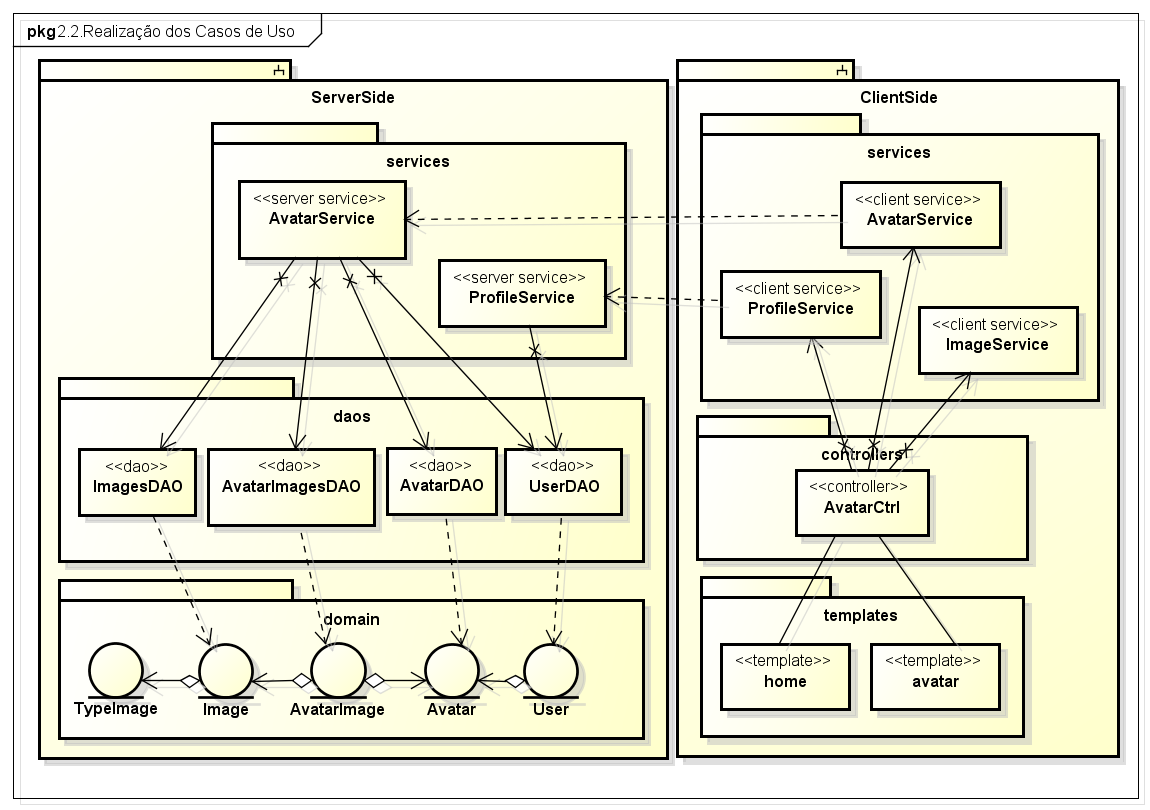
\includegraphics[width=33em]{figuras/avatarClasses.png}}
    \label{fig:avatarClasses}
\end{minipage}
\end{figure}

No lado do cliente, o objeto AvatarCtrl é responsável pela manipulação das imagens do avatar e dos eventos provindos da interação do usuário com a GUI. O AvatarService é responsável pela troca de dados com o servidor; o ImageService, pelo resgate das imagens do sistema de arquivos local para a aplicação e o ProfileService, pela troca de dados relativos ao usuário, entre eles, o nível, que define quais peças do avatar estarão disponíveis para customização. A visualização do avatar (sem opções de customização) é localizada na tela inicial do sistema.
\par
No lado do servidor, os objetos \textit{server services} interpretam os dados enviados pelo cliente, garantem a integridade desses dados e os encaminham para os DAOs, os quais salvam cada peça do avatar em seu devido local no banco de dados. 

\section{Módulo de Desafios}
O módulo de desafios contemplará uma série de tarefas propostas ao usuário que, quando cumpridas, o recompensam com itens para customizar o avatar. Em primeiro momento, haverá quatro desafios, cada um disponível para um nível. Quando os desafios de um nível são completados, o nível do usuário aumenta em um.
\par
Para a elaboração dos desafios foram pesquisados modelos de treinamento de ciclismo, o livro "The Cyclist's Training Bible" de Joe Friel\citeyearpar{friel2012cyclist} possui uma coletânea de planos e técnicas de ciclismo, baseados no tempo de atividade, cadência e potência. No entanto, a cadência e potência necessitam de equipamentos específicos para serem medidas e o tempo não garante que o usuário estava em movimento durante o monitoramento da atividade. Por estes motivos, decidiu-se utilizar a variável \textbf{distância} como requisito nos desafios.
\par
A quantidade de distância para cumprir o primeiro desafio baseou-se em um dos principais segmentos de ciclismo da cidade de Porto Alegre, o trajeto Ipiranga-Hipódromo, disponível no aplicativo Strava (Figura \ref{fig:segment}). Este trajeto tem 5.7km.

\begin{figure}[h]
\begin{minipage}{1.0\textwidth}
    \captionof{figure}{Ipiranga-Hipódromo: Segmento de pedalada em Porto Alegre, Rio Grande do Sul, Brazil.}
    \centerline{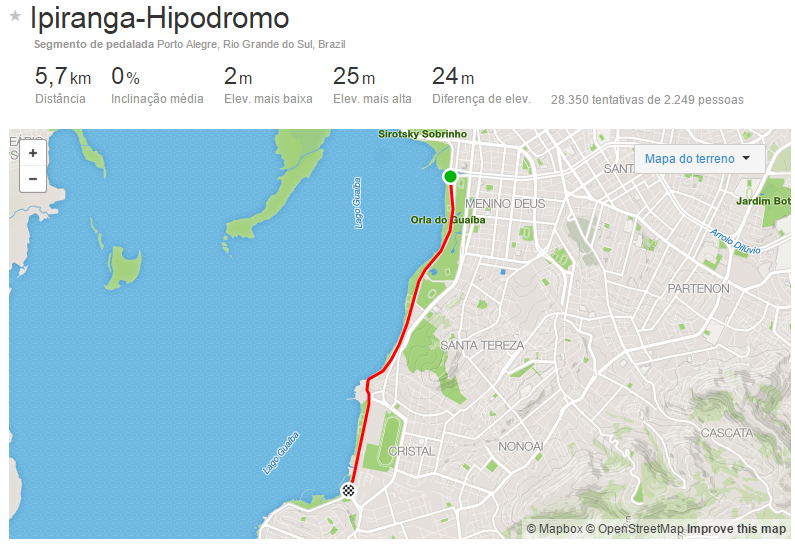
\includegraphics[width=25em]{figuras/stravaSegment.png}}
    \label{fig:segment}
\end{minipage}
\centerline{Fonte: \textit{Print screen} da aplicação Strava.}
\end{figure}

Cada desafio aumenta exponencialmente a quantidade de distância necessária. O desafio de nível 1, para ser cumprido, necessita de pelo menos uma pedalada em um percurso com distância equivalente a do seguimento Ipiranga-Hipódromo; o de nível 2, quatro pedaladas; de nível 3, 10 pedalas e de nível 4, 20 pedaladas, este é o último desafio pois o nível 5 é o último. Os desafios estão descritos na tabela \ref{tab:quests}, assim como suas recompensas e níveis necessários.

\begin{table}
\centering
\caption{Desafios propostos nos níveis do Pedal-to-Play}
\label{my-label}
\begin{tabular}{ccc}
\rowcolor[HTML]{C0C0C0} 
\multicolumn{1}{c|}{\cellcolor[HTML]{C0C0C0}{\color[HTML]{FFFFFF} \textbf{Nível}}} & \multicolumn{1}{c|}{\cellcolor[HTML]{C0C0C0}{\color[HTML]{FFFFFF} \textbf{Requisitos do Desafio}}} & {\color[HTML]{FFFFFF} \textbf{Recompensas}} \\ \hline
\multicolumn{1}{c|}{1}                                                             & \multicolumn{1}{c|}{Acumular 5 km de pedalada.}                                                    & Luvas e BMX.                                 \\ \hline
\multicolumn{1}{c|}{2}                                                             & \multicolumn{1}{c|}{Acumular 20 km de pedalada.}                                                   & Sapatos e Mountain.                       \\ \hline
\multicolumn{1}{c|}{3}                                                            & \multicolumn{1}{c|}{Acumular 50 km de pedalada.}                                                   & Óculos e Road bike.                           \\ \hline
\multicolumn{1}{c|}{4}                                                             & \multicolumn{1}{c|}{Acumular 100 km de pedalada.}                                                  & Vestimenta e Triathlon bike.                 \\ \hline
\end{tabular}
\label{tab:quests}
\end{table}

\section{Compilação para Mobile e Hospedagem do Web Service}
Outras atividades que demandaram um tempo considerável da implementação foram a adequação do projeto para a plataforma Android (usando Cordova) e a hospedagem do \textit{web service}.
\par
Para compilação do projeto em uma aplicação \textit{mobile} foram analisados os \textit{frameworks} Ionic\footnote{\url{http://ionicframework.com/}} e Phonegap\footnote{\url{http://phonegap.com/}}. Ambos são construídos em cima da plataforma Cordova. O Phonegap foi a primeira distribuição do Cordova, enquanto o Ionic é uma distribuição mais recente. O diferencial do Ionic é o uso em conjunto do \textit{framework} AngularJS. Devido a esta característica, foi cogitado utilizar o Ionic para desenvolvimento da versão \textit{mobile} do Pedal-to-Play, pois o lado cliente do sistema é baseado em AngularJS. Todavia, o Ionic, além de um \textit{framework} Cordova, também é um \textit{framework} de CSS. Ele possui estilos próprios para desenvolvimento da GUI e estes estilos não eram interessantes para o Pedal-to-Play, pois são específicos para \textit{mobile} e não se ajustam corretamente em telas grandes, como a de um computador pessoal. Sendo um dos objetivos deste projeto ser multiplataforma, essa característica do Ionic tornaria-se uma desvantagem. Então, optou-se por utilizar o Phonegap e o Bootstrap para os estilos da GUI, o qual tem boa responsividade para qualquer tamanho de tela. 
\par
Em conjunto com o Bootstrap, utilizou-se o \textit{plugin} Jasny-Bootstrap\footnote{\url{http://www.jasny.net/bootstrap/}}, para criação do menu de navegação lateral entre as telas do sistema. Este menu aparece somente em telas com largura menor que 768 \textit{pixels}. 
\par
Para captura de eventos \textit{touch sreen} nos dispositivos \textit{mobile}, o Pedal-to-Play também agregou o módulo de AngularJS, ngTouch\footnote{\url{https://docs.angularjs.org/api/ngTouch}}. E para iconografia, a biblioteca Font Awesome\footnote{\url{https://fortawesome.github.io/Font-Awesome/}} 
\par
Em relação à hospedagem do \textit{web service}, foi necessário conFigurar o servidor para suportar requisições de domínio cruzado (CORS) e um aprofundamento no \textit{framework} Slim. Para conFiguração do CORS utilizou-se o tutorial de Remy Shrap \citeyearpar{remyCors} e o tutorial do Apache sobre o arquivo “.htaccess” \citeyearpar{htaccess}.
\par
O \textit{web service} foi hospedado em um plano gratuito na plataforma Openshift. Também foi cogitado o uso do serviço do Hostinger. No entanto, as características do Openshift mostraram-se mais interessantes, entre elas: servidor com máquina virtual Linux; suporte a várias linguagens de programação, \textit{frameworks}, banco de dados e servidores Web; integração com Git; servidores fisicamente localizados na América escalonamento automático da aplicação e acesso SSH.

\section{Softwares Terceiros Utilizados}
Além dos módulos de AngularJS, dos \textit{plugins} de Cordova e de Bootstrap citados anteriormente, o Pedal-to-Play também fez uso dos seguintes softwares de terceiros para o desenvolvimento da solução técnica:

\begin{itemize}
\item UI Router: módulo de AngularJS para gerenciamento das URLs e transições entre as páginas Web do sistema\footnote{\url{http://angular-ui.github.io/ui-router/site/\#/api/ui.router}}; 
\item Gap Debug: ferramenta para \textit{debug} de aplicações desenvolvidas em Phonegap diretamente nos dispositivos \textit{mobile}\footnote{\url{https://www.genuitec.com/products/gapdebug/}};
\item Visual Studio Code: editor de texto da Microsoft com vários recursos para desenvolvimento de aplicações em JS\footnote{\url{https://code.visualstudio.com/}};
\item Netbeans IDE: ambiente de desenvolvimento com suporte a várias linguagens. Utilizou-se este \textit{software} para desenvolvimento do \textit{web service}\footnote{\url{https://netbeans.org/}};
\item Firefox Developer Edition: navegador baseado no Mozilla Firefox com recursos auxiliares para desenvolvimento de aplicações Web\footnote{\url{https://www.mozilla.org/pt-BR/firefox/developer/}}.
\end{itemize}

\section{Conclusões}
Neste capítulo foi apresentado como decorreu a implementação dos módulos de Autenticação, Avatar, Monitoramento de pedaladas e Desafios. Assim como o resumo de atividades e recursos que envolveram o desenvolvimento destes módulos, tais como a compilação do projeto para Mobile, a hospedagem do servidor e os \textit{softwares} terceiros agregados ao projeto ou que serviram de apoio ao desenvolvimento dele.
\par
O módulo de integração com redes sociais não foi desenvolvido, embora constasse no planejamento do projeto. O calendário planejado era utópico comparado ao tempo que foi necessário de fato para o desenvolvimento de cada módulo. O gráfico presente na Figura \ref{fig:gantt} ilustra a fase de implementação e apresenta quanto tempo utilizou-se para desenvolvimento de cada módulo e atividades relacionadas, totalizando 99 dias.

\begin{figure}[h]
\begin{minipage}{1.0\textwidth}
    \captionof{figure}{Gráfico de Gantt referente ao período de implementação.}
    \centerline{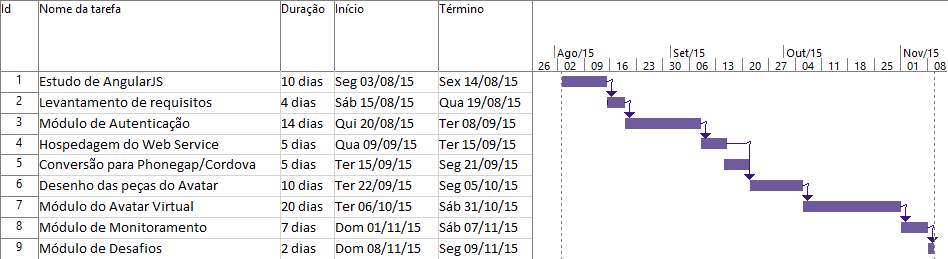
\includegraphics[width=35em]{figuras/ganttDesenv.png}}
    \label{fig:gantt}
\end{minipage}
\end{figure}

%A arquitetura final do sistema, após a fase de implementação, está %representada na \ref{fig:arquiteturaFinal}.
%
%\begin{figure}
%\begin{minipage}{1.0\textwidth}
%    \captionof{figure}{Arquitetura final do sistema.}
%    \centerline{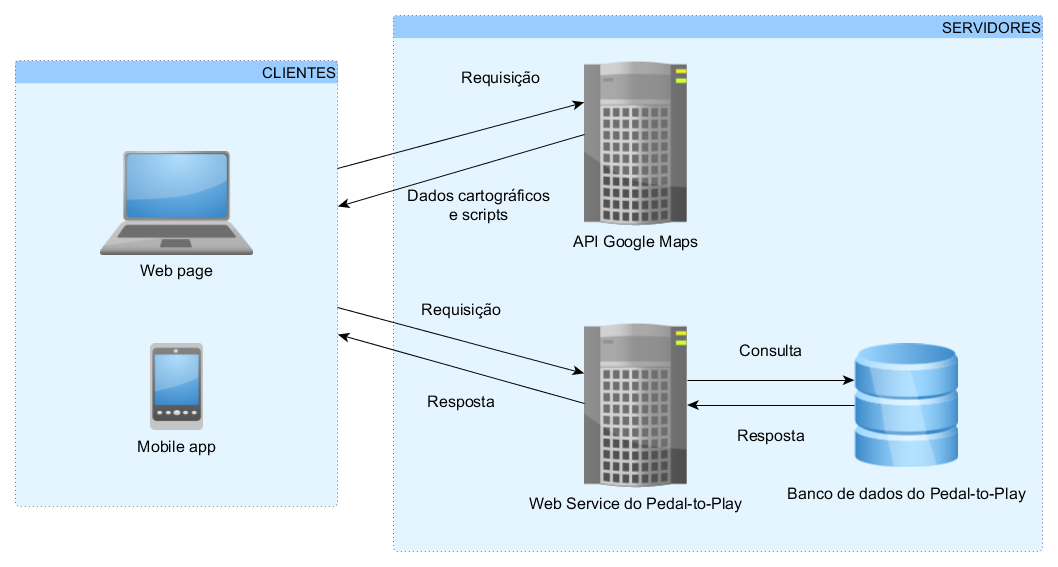
\includegraphics[width=30em]{figuras/arquiteturaFinal.png}}
%    \label{fig:arquiteturaFinal}
%\end{minipage}
%\end{figure}

O próximo capítulo apresentará os resultados obtidos a partir dos módulos implementados. Incluindo \textit{print screens} do sistema e a descrição dos testes de monitoramento de pedaladas reais.